\documentclass[10pt]{article} % 5p gir 2 kolonner pr side. 1p gir 1 kolonne pr side.

\usepackage[T1]{fontenc}
\usepackage[]{lmodern}
\usepackage[utf8]{inputenc}
\usepackage[english]{babel} % Tilpasning til norsk.
%\usepackage[demo]{graphicx} % For ?? inkludere figurer.

\usepackage{lipsum}
\usepackage{booktabs}
\usepackage{csquotes}


\usepackage{amsmath,amsfonts,amssymb} % Ekstra matematikkfunksjoner.
\allowdisplaybreaks[1]

\DeclareMathOperator{\lcm}{lcm}
\newcommand{\kortlinje}{\vspace{-0.25cm}}

\usepackage{amsthm}

\newtheorem{lemma}{Lemma}
\newtheorem{proposition}{Proposition}
\newtheorem{definition}{Definition}

\usepackage{imakeidx}
\makeindex[columns=3, title=Alphabetical Index]

\usepackage[dvipsnames*,
		    svgnames]{xcolor}       % more colors

\usepackage{graphicx}

\usepackage{tikz}
\usetikzlibrary{trees}
    
\usepackage{caption}
% Disse kommandoene kan gj??re det enklere for LaTeX ?? plassere figurer og tabeller der du ??nsker.
\usepackage{subcaption}

\usepackage{fullpage}


%%%%%%%%%%%%%%%%%%%%%%%%%%%%%%%%%%%%%%%%%%%%%%%%%%%%%%%%%%%%%%%

\usepackage{siunitx} % Må inkluderes for blant annet å få tilgang til kommandoen \SI (korrekte måltall med enheter)
\sisetup{exponent-product = \cdot}      % Prikk som multiplikasjonstegn (i steden for kryss).
\sisetup{output-decimal-marker  =  {,}} % Komma som desimalskilletegn (i steden for punktum).
\sisetup{separate-uncertainty = true}   % Pluss-minus-form på usikkerhet (i steden for parentes).
\sisetup{table-number-alignment = right ,
        table-format=2.3,
        per-mode=symbol}
\sisetup{math-micro=\text{µ},text-micro=µ}
\usepackage{textcomp}

%%%%%%%%%%%%%%%%%%%%%%%%%%%%%%%%%%%%%%%%%%%%%%%%%%%%%%%%%%%%%%%

\usepackage{minted}
\usemintedstyle{pastie}

\newminted{python}{fontsize=\small}

\usepackage[framemethod=TikZ]{mdframed}


\newenvironment{ProjectEuler}[2][]{%

\setcounter{section}{#2}

\addcontentsline{toc}{section}{Project Euler~#2:~#1}
\ifstrempty{#1}%
{\mdfsetup{%
frametitle={%
\tikz[baseline = (current bounding box.east), outer sep = 0pt]
\node[anchor = east, rectangle, fill = blue!20]
{\strut Project Euler~#2};}}
}%
{\mdfsetup{%
frametitle={%
\tikz[baseline = (current bounding box.east),outer sep = 0pt]
\node[anchor = east, rectangle, fill = blue!20]
{\strut \hypersetup{urlcolor = {}}\href{https://projecteuler.net/problem=#2}{Project Euler~#2:~#1}\hypersetup{urlcolor = cyan}};}}%
}%
\mdfsetup{innertopmargin=10pt, linecolor=blue!20,%
linewidth = 2pt, topline = true,%
frametitleaboveskip=\dimexpr-\ht\strutbox\relax
}
\begin{mdframed}[]\relax%
\label{PE-#2}}{\end{mdframed}}


%%%%%%%%%%%%%%%%%%%%%%%%%%%%%%%%%%%%%%%%%%%%%%%%%%%%%%%%%%%%%%%


\def\figureautorefname{figur}  % Får hyperlenker til figurer på norsk
\def\tableautorefname{tabell}   % Får hyperlenker til tabeller på norsk
\def\equationautorefname{likning}

% Centeres figures automagically
\makeatletter
\g@addto@macro\@floatboxreset\centering
\makeatother

			
%%%%%%%%%%%%%%%%%%%%%%%%%%%%%%%%%%%%%%%%%%%%%%%%%%%%%%%%%%%%%%%%%%%%%%%%%

% Hyper references

%%%%%%%%%%%%%%%%%%%%%%%%%%%%%%%%%%%%%%%%%%%%%%%%%%%%%%%%%%%%%%%%%%%%%%%%%

\usepackage{hyperref}
\hypersetup{colorlinks=true,
            pdfmenubar=false,
            pdfstartview={FitH},
            linktoc = all,
            urlcolor = purple,
            citecolor = black,
            linkcolor = {}}

\usepackage[nameinlink]{cleveref}


%%%%%%%%%%%%%%%%%%%%%%%%%%%%%%%%%%%%%%%%%%%%%%%%%%%%%%%%%%%%%%%%%%%%%%%%%

% Bibliography

%%%%%%%%%%%%%%%%%%%%%%%%%%%%%%%%%%%%%%%%%%%%%%%%%%%%%%%%%%%%%%%%%%%%%%%%%

\usepackage[numbers]{natbib}
\usepackage{chapterbib}

%%%%%%%%%%%%%%%%%%%%%%%%%%%%%%%%%%%%%%%%%%%%%%%%%%%%%%%%%%%%%%%%%%%%%%%%%



\usepackage{multicol}

%Defines the linkcolor 
\newcommand{\link}{NavyBlue}

\usepackage[nameinlink]{cleveref}

\creflabelformat{equation}{#2(\textcolor{\link}{#1})#3}
\creflabelformat{table}{#2\textcolor{\link}{#1}#3}
\creflabelformat{figure}{\!#2\textcolor{\link}{#1}#3}

\title{Project Euler \\ - Prematurely optimized and Overengineered }
\author{Øistein Søvik}

\begin{document}

\maketitle

\cleardoublepage

	\include{Preface}
	
\setcounter{tocdepth}{1}
\tableofcontents

	  \begin{ProjectEuler}[Multiples of $3$ and $5$]{1}

If we list all the natural numbers below 10 that are multiples of $3$ or $5$, we get $3$, $5$, $6$ and $9$. The sum of these multiples is $23$.
\medskip

\noindent Find the sum of all the multiples of $3$ or $5$ below $1000$.

\end{ProjectEuler}

It is straight forward to iterate over the first $1000$ numbers and check for divisibility.

\begin{pythoncode}
	def divisible_by_3_or_5(limit = 1000):
	    count = 0
	    for num in xrange(1, limit):
	        if num%3 == 0 or num%5 == 0:
	            count += num
	    return count
\end{pythoncode}
%
The code above takes on average \SI{12}{\micro\s} to run. Well under the arbitary \SI{1}{\s} rule. However we can do better, a small improvement
is to allow for different numbers than $3$ or $5$ and also allow for a customizable range. 
%
\begin{pythoncode}
	def numbers_divisible(divisors=[3, 5], start=0, stop=100):
	    count = 0
	    for num in xrange(start, stop):
	        for d in divisors:
	            if num % d == 0:
	                count += num
	                break
	    return count
\end{pythoncode}
%
It could seem the above code is quite fast however running \verb|numbers_divisible([3, 5], 0, 10**9)| takes about \SI{450}{\s} to run. 
This is painfully slow, but also expected since the code runs in $\mathcal{O}(n)$. As we shall see we can make the code run in constant time. 
%
\paragraph*{Improved algorithm for two numbers}
%
The first step is to count the number of numbers divisible by 3, then 5. 
However adding these two will give the incorrect answer, we can see why by listing the first few numbers.
$[3, 6, 9, 15]$ and $[5, 10, 15]$. So every number which is divisble by 3 and 5 is counted twice. \Cref{fig:PE1-venn-2} visualizes this.
%
\begin{figure}[h!tbp]
	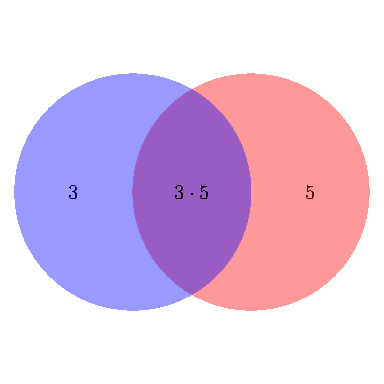
\includegraphics[scale=1, trim={0.25cm 1.25cm 0.25cm 1.25cm}, clip]{Images/Project-Euler-001-Venn-Diagram-2.pdf}
	\caption{}
	\label{fig:PE1-venn-2}
\end{figure}
% 
\begin{pythoncode}
    div_by_3 = [3*i for i in range(int(999/3))]
    div_by_5 = [5*i for i in range(int(999/5))]
    div_by_3_and_5 = [15*i for i in range(int(999/15))]
    return div_by_3 + div_by_5 - div_by_3_and_5
\end{pythoncode}
%
This is slightly faster than the naive implementation. However we can find a closed formula for the number of numbers
divisble by 3, or any other number. The closed formula for the first $n$ numbers are\footnote{See \url{https://en.wikipedia.org/wiki/1_\%2B_2_\%2B_3_\%2B_4_\%2B_\%E2\%8B\%AF} for further details.}
%
\begin{align*}
	0 + 1 + \cdots + (m-1) + m = \frac{m(m+1)}{2}
\end{align*}
%
To find the sum of the natural numbers starting at some number $n$ up to some number $m$ we can subtract the sum of numbers up to $n-1$. 
%
\begin{align*}
	  n + (n+1) + \cdots +(m-1) + m
	= \frac{m(m+1)}{2} - \frac{(n-1)n}{2}
	= \frac{1}{2}(m+n)(m-n+1)
\end{align*} 
Since $3 + 6 + 9 + 12 + \cdots = 3 (1 + 2 + 3 + \cdots)$ we can just multiply the above formula by $3$ to sum the multiples of $3$. 
However we have to make sure we are not multiplying numbers larger than $1000$. So we can not let $m$ be $1000$ and sum up a thousand multiples of $3$.
The largest of these would be $3 \cdot 1000$ which is 3 times as large as the limit. One solution is to take $m = 999/3$. 


If we are summing over multiples of $k$, then the upper limit would be $(text{limit}-1)/k$ rounded down.

One problem with this code can be seen with the $[6, 9]$. The code removes multiples of $6 \cdot 9 = 56$ however the 
first value that is counted twice is $18$. One way to solve this is to divide the product by the lowest common divisor (gcd). 
So we would have $56/\gcd(6,9) = 56/3 = 18$.
%	
\begin{pythoncode}
	from fractions import gcd
	def sum_divisible_by_k(k, start, limit):
    	stop = int((limit-1)/float(k))
    	return k*(stop+start)*(stop-start+1)/2

	def divisible_by_a_or_b(num_a, num_b, start=0, limit=100):
	    divisors = [num_a, num_b]
	    total = 0
	    for divisor in divisors:
	        total += sum_divisible_by_k(divisor, start, limit)
	    product = divisors[0]*divisors[1]/gcd(a, b)
	    return total - sum_divisible_by_k(product, start, limit)
\end{pythoncode}
%
For values up to $10^5$ the improved version runs around $4500$ times faster. However as stated this function runs in constant time
so a speed comparison is not really necessary. We have now done the \emph{silly} speed improvements. 
%
\paragraph*{More than two numbers}

There are some bumps to work out for the generalized version. We shall start looking into the simplest case $[2, 3, 5]$. We can visualize the double counting as follows
%
%
\begin{figure}[h!tbp]
	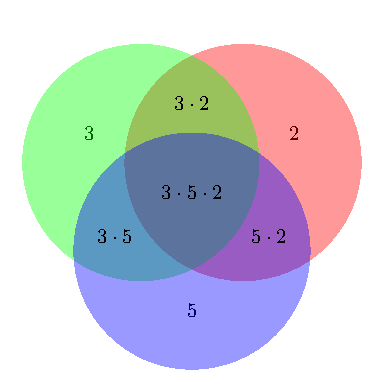
\includegraphics[scale=1, trim={0.25cm 0.25cm 0.25cm 0.75cm}, clip]{Images/Project-Euler-001-Venn-Diagram-3.pdf}
	\caption{}
	\label{fig:PE1-venn-3}
\end{figure}
% 
As we can see from \cref{fig:PE1-venn-3} we have to remove the multiples of $2\cdot 3, 2\cdot 5$ and $3 \cdot 5$. However removing these
will remove too many values. As an exercise you can check that $60$ is missing if we do not add the multiples of $2 \cdot 3 \cdot 5$. 

The next problem to work out is multiples. Take $[2, 3, 8]$, there is no need to add $8$ once we have added $2$. The following code
removes all multiples, all doubles and sorts the divisors. 
%
\begin{pythoncode}
def remove_multiples(divisors):
    new_divisors = []
    divisors = sorted(set(divisors))
    for divisor in divisors:
        if not any(divisor % d == 0 for d in new_divisors):
            new_divisors.append(divisor)
    return new_divisors
\end{pythoncode}
%
The final problem is that we still have to divide by the greatest common divisor. However we now have to perform this on a list of numbers.
Luckily the $\gcd$ functions is additive so that $\gcd(a, b, c) = \gcd( \gcd(a, b), c)$. Since we this be done quite a few times
I will use memoization and save some calculation. 
%
\begin{pythoncode}
gcd_dict = defaultdict(int)
def gcd_list(numbers):
    numbers_len = len(numbers)
    a = perm[0]
    for i in range(1, numbers_len):
        b = perm[i]
        if gcd_dict[(a, b)] == 0:
            gcd_dict[(a, b)] = gcd(a, b)
        a = gcd_dict[(a, b)]
    return a
\end{pythoncode}
%
The final code in all it's glory can now be written as
%
\begin{pythoncode}
def sum_divisible_ny_numbers(numbers, start, stop):
    divisors = remove_multiples(numbers)

    total = 0
    for divisor in divisors:
        total += sum_divisible_by_k(divisor, start, stop)

    k = -1
    for i in range(2, len(divisors)+1):
        for perm in combinations(divisors, i):
            product = reduce(mul, perm)/gcd_list(perm)
            total += k*sum_divisible_by_k(product, start, stop)
        k *= -1
    return int(total)
\end{pythoncode}
%
The running time of this algorithm is $\mathcal{O}(2^{d})$ where $d$ is the number of unique numbers to check for. This is also the reason we take time to remove duplicates
and multiples of values. 

% \bibliographystyle{amsalpha}
% \bibliography{../REFF}

%%% Local Variables: 
%%% mode: latex
%%% TeX-master: "../Project-Euler.tex"
%%% End: 
	
	  \begin{ProjectEuler}[Even Fibonacci numbers]{2}
	Each new term in the Fibonacci sequence is generated by adding the previous two terms. By starting with $1$ and $2$, the first $10$ terms will be:
	%
	\begin{align*}
		1, 2, 3, 5, 8, 13, 21, 34, 55, 89, \ldots
	\end{align*}
	%
	By considering the terms in the Fibonacci sequence whose values do not exceed four million, find the sum of the even-valued terms.
\end{ProjectEuler}
\begin{pythoncode}
	sum(int(.5+5**(-.5)*(.5+.5*5**.5)**(3*n)) for n in 
	range(100) if int(.5+5**(-.5)*(.5+.5*5**.5)**(3*n)) < 4*10**6)
\end{pythoncode}
This is one of my favourite problems and as a teaser one of the solution can be written as
%
\begin{pythoncode}
	def sum_even_fibonacci(limit):
    	a, b = 0, 2
    	while b < limit:
        	a, b = b, 4 * b + a
    	return (a + b - 2) / 4
\end{pythoncode}
%
However to understand how this code works we have to go pretty far down the rabbit hole. A warning before we start: this problem
is very easy to solve under \SI{1}{s}, and any improvements beyond this is purely for the amusement of the Author. By the end
we will have developed a method to find the sum of all even Fibonacci numbers under $10^{\num{10 000}}$ in about a \SI{1}{\ms}.
\begin{definition}
	the Fibonacci numbers are the numbers in the following integer sequence, called the Fibonacci sequence:
	\kortlinje
	%
	\begin{align*}
		0,\;1,\;1,\;2,\;3,\;5,\;8,\;13,\;21,\;34,\;55,\;89,\;144,\; \ldots
	\end{align*}
	%
	The numbers have in common that each subsequent number is the sum of the previous two. In mathematical terms we can define the Fibonacci numbers as:
	\begin{align}
	\label{eq: P01 F_n=F_n-1+F_n-2}
		F_{n} = F_{n-1} + F_{n-2}
	\end{align}
	with initial conditions $F_0 = 0$ and $F_1 = 1$.
\end{definition}
%
Note that this definition differs slightly from the proposed by Project Euler. The difference is that our indices
is shifted $n \to n+2$ such that $F_{\text{PE} n} = F_{n + 2}$. The  only reason for this is that it leads to slightly nicer notation later on.

The definition above leads us straight into the following code
\begin{pythoncode}
	def fib(n):
        if n < 2:
            return n
        else:
            return fib(n-1) + fib(n-2)
            
	def sum_even_fib_naive(limit):
	    n = total = 0
	    while fib(n) < limit:
	        n += 1
	        if fib(n) % 2 == 0:
	            total += fib(n)
	    return total
\end{pythoncode}
%
This is so far the slowest solution I have yet written to a Project Euler problem. To just see how slow it is we can measure 
the number of times \verb|fib| is called. To evaluate $F_5$ we have to call our function $35$ times! See \cref{fig: PE02-fib5-tree}
for a visualization of this. If you have a bit of sparetime try to see how big this tree gets for $F_6$, and if you 
have a couple of lifetimes to spare you can verify that \verb|f(33)| makes \num{29860703} function calls.
\begin{figure}[h!tbp]
	\centering
	\begin{tikzpicture}[level distance=1cm,
		level 1/.style={sibling distance=6cm},
		level 2/.style={sibling distance=3cm},
	 	level 3/.style={sibling distance=2cm}]
	 	\node {$F_5$}
	    	child {node {$F_4$}
	      		child {node {$F_3$}
					child {node {$F_2$}
						child {node {$F_1$}}
						child {node {$F_0$}}
					}
					child {node {$F_1$}}      
				}
				child {node {$F_2$}
		      		child {node{$F_1$}}
		      		child {node{$F_0$}}
	    		}
	    	}	    
		    child {node {$F_3$}
				child {node {$F_2$}
					child {node {$F_1$}}
					child {node {$F_0$}}
				}
				child {node {$F_1$}}      
		      };
	\end{tikzpicture}
	\caption{Shows the computations needed to evaluate $F_5$.}
	\label{fig: PE02-fib5-tree}
\end{figure}
%
This is the reason our code is so slow, and it can be shown that \verb|fib(n)| grows as $\mathcal{O}(\phi^n)$. Here $\phi$ is the golden ratio and
shortly see how this number plays a role in our calculations. One method to fix the problem with recursively calling our function is
to store the previously calculated values in memory
%
\begin{multicols}{2}
\begin{pythoncode}
	def fib_memo(n):
	    pad = {0:0, 1:1}
	    def func(n):
	        if n not in pad:
	            pad[n] = func(n-1) + func(n-2)
	        return pad[n]
	    return func(n)
\end{pythoncode}
\vfill
\columnbreak
\begin{pythoncode}
	from functools import lru_cache
	
	@lru_cache(maxsize=None)
	def fib(n):
	    if n < 2:
	        return n
	    return fib(n-1) + fib(n-2)
\end{pythoncode}
\end{multicols}
%
\textbf{Note:} If you are using Python 2.7 you need to use \verb|from functools32 import lru_cache| to use \verb|@lru_cache|. Both of
these functions speeds up \verb|sum_even_fib_naive| dramatically. However the drawback of using memoization is that it needs to store
a large number of values and thus is not very memory efficient. In this problem however memory is not a concern since to obtain
the solution we only need to store 32 values in memory. 
%
On the other hand it is a good practice not to hog more memory than needed and in this problem it is easy to do so. \Cref{eq: P01 F_n=F_n-1+F_n-2}
is know as a \emph{second order linear homogeneous recurrence relation}. That was a bit of a mouthful, but it basically means we can find a
closed form for the $n$th Fibonacci number. One way to find the solution to these equations is to simply \emph{guess}. 
You are free to try $f(n) = An + B$, $f(n) = A n^2 + B n + C $ or any other polynomial. However none of these attempts work out. For
recurrence relations our first guess is usually on the form $f(n) = A \cdot P^n$, inserting this in \cref{eq: P01 F_n=F_n-1+F_n-2} gives
%
\begin{align}
	\label{eq: PE02 A(P^n-P^(n-1)-P^(n-2))}
	A \cdot (P^n - P^{n-1} - P^{n-2}) = 0
\end{align}
%
For the relation to hold the left-hand side to be zero for all values of $n$ either $A$ or $P^n - P^{n-1} - P^{n-2}$ has to be zero.
$f(n) = 0$ satisfies $F_n = F_{n-1} - F_{n-2}$, however it is obviously not the solution we are looking for. Hence
we assume that $A \neq 0$, and we can safely divide \cref{eq: PE02 A(P^n-P^(n-1)-P^(n-2))} by $A$. In the same vein we also
multiply the equation by $P^{2-n}$
\begin{align*}
	P^2 - P - 1 = 0
\end{align*}
% 
This is called the \emph{characteristic polynomial} to our recurrence relation. The roots of this equation gives us 
the valid values for $P$ such that $f(n) = A \cdot P^n$ satisfies \cref{eq: P01 F_n=F_n-1+F_n-2}. 
%
\begin{align*}
	P = 0 \vee P = \frac{1 \pm \sqrt{5}}{2}
\end{align*}
%
Again $P = 0$ is the \emph{trivial} solution. I will leave it to you to verify that $f(n) = A [ (1 + \sqrt{5})/2]^n$ satisfies
$f(n) = f(n-1) + f(n-2)$. There is a small problem with our solution however, even though it satisfies the recurrence relation 
the \emph{initial-values} are wrong. We need $f(0)=0$, but then $f(0) = A$, hence $A = 0$ and we are again left with the trivial solution.

For a moment assume that both $f(n) = A P^n$ and $g(n) = B Q^n$ satisfies \cref{eq: P01 F_n=F_n-1+F_n-2}, then $h(n) = A P^n + B Q^n$
will also satisfy the equation. Said more plainly \emph{a sum of solutions is also a solution}. Our next guess therefore becomes
%
\begin{align*}
	f(n) = A \left( \frac{1 + \sqrt{5}}{2} \right)^n + B \left( \frac{1 - \sqrt{5}}{2} \right)^n
\end{align*}
%
What remains is finding $A$, and $B$ such that $f(0) = 0$ and $f(1) = 1$. This leads to the following system of equations
%
\begin{align*}
	A + B = 0 \quad \text{and} \quad 
	A \left( \frac{1 + \sqrt{5}}{2} \right) + B \left( \frac{1 - \sqrt{5}}{2} \right) = 0
\end{align*}
%
Solving this system is quite trivial and yields $A = 1/\sqrt{5}$ and $B = -A = -1/\sqrt{5}$. 
%
\begin{align*}
	F_n = \frac{1}{\sqrt{5}} \left( \frac{1 + \sqrt{5}}{2} \right)^n - \frac{1}{\sqrt{5}} \left( \frac{1 - \sqrt{5}}{2} \right)^n
\end{align*}
%
This equation can be written in a varity of ways and I have collected a handful below
\begin{align}
\label{eq: PE02 closed-form-fibonacci}
	   F_n 
	= \frac{\phi^n - \psi^n}{\phi - \psi} 
	= \frac{\phi^n - \psi^n}{\sqrt{5}}
	= \frac{\phi^n - (-\phi)^{-n}}{\sqrt{5}}
\end{align}
The notation $\phi = (1 + \sqrt{5})/2$ and $\psi = (1 - \sqrt{5})/2$ was used for convenience sake\footnote{Know as the golden ratio}.
Proving the last relation implies proving $\psi = -1/\phi \ \Longrightarrow \ \psi^n = (-1/\phi)^n = \phi^{-n}$ is left as a small exercise.  
The implications this has is that $(-\phi)^{-n}$ quickly diminishes $(-\phi)^{-10} \approx \num{0.00813}$. Hence we can implement the $F_n$
function as $F_n = \text{ceil}( \phi^n / \sqrt{5})$.
%
\begin{pythoncode}
	SQRT_5 = 5**0.5
	PHI = 0.5*(1 + SQRT_5)
	def fib_exact(n):
	    return int(0.5 + (PHI**n)/SQRT_5)
\end{pythoncode}
%
Where \verb|int(0.5+num)| was used to round up, since $\text{floor}(x+0.5) = \text{ceil}(x)$. At a first glance this seems like the perfect solution
as it runs in constant running time and for our problem it works without quirks. However exponentiation with decimal numbers is very prone to rounding errors.
Checking the accuracy of this function one can see that it starts deviates from the actual Fibonacci numbers after $n = 71$. 
For now I present an alternative. The following code is a simple exact way to generate the fibonacci numbers without relying on recursion nor memoization. 
%
\begin{multicols}{2}
\begin{pythoncode}
	def fib_generator():
	    F0, F1 = 0, 1
	    while True:
	        yield F0
	        F1, F0 = F1 + F0, F1
\end{pythoncode}
\vfill
\columnbreak
\begin{pythoncode}
def sum_even_fibbonaci(limit):
    total = 0
    for nth_fib in fib_generator():
        if nth_fib % 2 != 0: continue
        if nth_fib > limit: return total
        total += nth_fib
\end{pythoncode}
\end{multicols}
Even though the closed form could not be used our efforts have not been completely wasted. \Cref{eq: PE02 closed-form-fibonacci} gives
us an excellent starting point in figuring out how many terms we need. At first glance this seems complicated and for complete accuracy 
we should use a numerical method such as Newton-rhapson or the bisection method. However since $(-\phi)^{-n}$ diminishes so quickly a
 rough solution is just to ignore it. 
\begin{align*}
	M = F_{3n} 
	\ \Rightarrow \ 
	M \approx \frac{\phi^{3n}}{\sqrt{5}}
	\ \Rightarrow \
	n \approx \frac{1}{6} \log_\phi(5) + \frac{1}{3} \log_\phi(M)
\end{align*}
 %
Where $M$ denotes the largest $F_n$ we will allow. For every $M > 1$ the approximation is equal to the actual value rounded down. 
%
\begin{pythoncode}
	from math import log

	PHI = (1 + 5**0.5)/float(2)
	LOG_5 = log(5, PHI)/float(6)
	
	def largest_even_fib_index(n):
	    return int(LOG_5 + log(n, PHI)/float(3))
	
	def sum_even_fibbonaci_w_end(M):
	    F0, F1, total = 0, 1, 0
	    for _ in range(largest_even_fib_index(M)):
	        for _ in range(3):
	            F1, F0 = F1 + F0, F1
	        total += F0
	    return total
\end{pythoncode}
%
Note that even after all these efforts the running time of our algorithm is still the same. 
By writing out the first Fibonacci numbers we can see a pattern start to form
%
\begin{align*}
	\mathbf{0},   \; 1,     \; 1,  \; 
	\mathbf{2},   \; 3,     \; 5,  \; 
	\mathbf{8},   \; 13,    \; 21, \; 
	\mathbf{34} , \; 55,    \; 89, \; 
	\mathbf{144}, \; \ldots
\end{align*}
%
It seems that every third Fibonacci number is divisible by 3. We can write a short proof using induction to verify this suspicion.
We want to prove that $F_{3n}$ is divisible by $2$ for every $k \geq 0$.
%
\begin{proof}
The base case is that $F_0$ is divisible by $2$, which it is since $F_0 = 0$. 
Assume that there exists some $k$ such that $F_{3k}$ is divisible by $2$. We have to prove that this
implies that $F_{3(k+1)} = F_{3k+3}$ is divisible by $2$. 
%
\begin{align}
	\label{eq: PE02 F_3(k+1))=F_3k+2F_(3k+1)}
	F_{3+3k} = F_{2+3k} + F_{1+3k} 
			 = \left[ F_{3k+1} + F_{3k}  \right] + F_{3k+1} 
			 = F_{3k} + 2 F_{3k+1}
\end{align}
%
Where \cref{eq: PE02 F_n=F_n-1+F_n-2} wss used twice.
Since $F_{3k}$ is divisible by $2$ from the induction hypothesis and $2 F_{3+3k}$ is clearly divisible by $2$, the claim follows by induction.
\end{proof}
%
Since there is a closed form for the Fibonacci numbers, it is not unreasonable to think that there exists a similar
pattern for the even Fibonacci numbers, but how can we discover such a pattern? \Cref{eq: PE02 F_3(k+1))=F_3k+2F_(3k+1)}
gives us a starting point, since it has a relation between two even Fibonacci numbers: $F_{3(k+1}$ and $F_3k$. The
only thing that remains is to rewrite $2 F_{3k+1}$ as a sum of even Fibonacci numbers.
%
\begin{align*}
	    2F_{3k+1} 
	& = 2(F_{3k} + F_{3k-1}) \\
	& = 2F_{3k} + 2 F_{3k-1} \\
	& = 2F_{3k} + F_{3k-1} + F_{3k-2} + F_{3k-3} \\
	& = 3F_{3k} + F_{3(k-1)}
\end{align*}
%
Replacing $2 F_{3k+1}$ with $3 F_{3k} + F_{3(k-1)}$ in \cref{eq: PE02 F_3(k+1))=F_3k+2F_(3k+1)} gives us the following relation
\begin{align}
	\label{eq: PE02 F_3(k+1))=4F_3k+2F_3(k-1)}
	F_{3(k+1} = 4 F_{3k} + F_{3(k-1)}
\end{align}
This can also be written as $E(n) = 4 E(n-1) + E(n-2)$ when we let $E(n)$ denote the $n$th even Fibonacci number.
Interestingly enough \cref{eq: PE02 F_3(k+1))=4F_3k+2F_3(k-1)} also holds for the odd Fibonacci numbers, and 
one can prove that $F_n = 4F_{n-3} + F_{n-6}$ holds for every $n$. This however will be left as an exercise for the reader.
%
\begin{pythoncode}
	def sum_even_fast(limit):
	    a, b = 0, 2
	    total = 0
	    while b < limit:
	        total += b
	        a, b = b, 4 * b + a
	    return total
\end{pythoncode}
%
This code is much faster than our previous attempts, and could further be slightly optimized 
by using \verb|for _ in range(largest_even_fib_index(M)):| instead of \verb|while b < limit:|.

The next optimization is to find a closed form for the sum of the first n Fibonacci numbers. 
%
\begin{proposition}
	\begin{align*}
		  \sum_{i=0}^n F_{3i} 
		= \frac{F_{3n+2}-1}{2}
		= \frac{F_{3n} + F_{3n+2} - 2}{4}
	\end{align*}
\end{proposition}
%
\begin{proof}
	We will prove the first relation by induction, while the second is left as an excercise. 
	Base case: $F_{3\cdot0} = 0$ and $(F_{0+2}-1)/2 = 0$. Assume that 
	for some $k$ we have $\sum_{i=0}^k F_{3i} = \frac{F_{3k+2}-1}{2}$. We want to prove 
	that this implies that $\sum_{i=0}^{k+1} F_{3i} = \frac{F_{3(k+1)+2}-1}{2}$ holds. 
	\begin{align*}
		    \sum_{i=0}^{k+1} F_{3i}
		  = F_{3(k+1)} + \sum_{i=0}^{k} F_{3i} 
		& = F_{3(k+1)} + \frac{F_{3k+2}-1}{2} \ \leftarrow \ \text{used the induction hypothesis} \\
		& = \frac{F_{3(k+1)} + F_{3k+3} + F_{3k+2} - 1}{2} 
		  = \frac{F_{3(k+1)} + F_{3(k+1)+1} + - 1}{2} 
		  = \frac{F_{3(k+1)+2}-1}{2}
	\end{align*}
Since $F_{3k+3} + F_{3(k+1)}$ and $F_{3k+2} + F_{3k+3}=F_{3k+4}=F_{3(k+1)+1}$, this concludes the proof.
\end{proof}
%
\begin{pythoncode}
	def constant_even_fib(limit):
	    n = largest_even_fib_under_n(limit)
	    return (int(0.5+PHI**(3*n+2)/5**0.5)-1)/2
\end{pythoncode}
%
This is a rather neat code, however it still suffers from floating point errors, when the powers get too high.
Another solution is to find a closed formula for $E_n = 4 E_{n-1} + E_{n-2}$. Similar as we did in equation nigga we can guess that
$E_n = A \cdot P^n + B \cdot Q^n$, where $P$ and $Q$ are the roots of the characteristic polynomial $x^2 - 4x -1 = (x-2)^2 -5$. 
%
\begin{align*}
	E_n = A (2 + \sqrt{5})^n + B (2 - \sqrt{5})^n
\end{align*}
%
As before we can find the constants using $E_0 = 0$ and $E_1 = 2$.
%
\begin{align*}
	     E_n 
	& = \frac{1}{\sqrt{5}} (2 + \sqrt{5})^n - \frac{1}{\sqrt{5}} (2 - \sqrt{5})^n \\
	    \frac{E_n + E_{n+1}-2}{4}
	& = \frac{1}{4}\left( \frac{1}{\sqrt{5}} (2 + \sqrt{5})^n  + \frac{1}{\sqrt{5}} (2 + \sqrt{5})^{n+1}  - 2 \right) 
	  = \frac{1}{4\sqrt{5}} ( 3 + \sqrt{5} ) (2 + \sqrt{5})^{n} - \frac{1}{2}
\end{align*}
%
Since $\left| (2 - \sqrt{5})^n \right| < 1/2$ for all $n>1$, we only need to add the powers of $2 + \sqrt{5}$.
%
\begin{pythoncode}
def fib_sum_even_constant(limit):
    n = largest_even_fib_under_n(limit)
    return int(.5+5**(-.5)*(3+5**.5)*(2 + 5**.5)**n)/4
\end{pythoncode}
%
Which of these two algorithms if any do you think performs the best? Note that the \verb|-0.5| 
was dropped again because how Python performs rounding. This concludes how far we can go in constant time,
however we are not quite at the end of the road.
%
\subsection{Fibonacci in sublinear time}

If we want to generate the first $n$ Fibonacci numbers the fastest we 
can do is in polynomial time $\mathcal{O}(n)$. This is only natural since we have to iterate over every element.
%
However as we will see if we are only interested in a particular $F_n$ we do not need to generate
every $F_i$ where $0 \leq i \leq k$. There are many different ways to achieve this, I will briefly show three algorithms.

There have been many smaller improvements on the Lucas numbers and the matrix multiplication method. 
One is credited to \citeauthor{Takahashi} which proposed the following algorithm. 
%
\begin{pythoncode}
	def fib_takahashi(n):
	    if n == 0:
	        return n
	    F, L, sign, exp = 1, 1, -2, int(log (n,2))
	    mask = 2**exp
	    for i in xrange (exp - 1):
	        mask = mask >> 1
	        F2   = F**2
	        FL2  = (F + L)**2
	        F    = ((FL2 - 6*F2) >> 1) - sign
	        if n & mask:
	            temp = (FL2 >> 2 ) + F2
	            L     = temp + (F << 1)
	            F     = temp
	        else:
	            L    = 5*F2 + sign
	        sign = -2 if n & mask else 2
	    if n & (mask >> 1) == 0:
	        return F * L
	    else:
	        return ((F + L) >> 1) * L - (sign >> 1)
\end{pythoncode}
%
I will not go into details on how the code works as this is explained much better than I can in his paper, see \cite{Takahashi}.

\bibliographystyle{plainnat}
\bibliography{../REFF}
	
	  
\begin{ProjectEuler}[Largest prime factor]{3}
The prime factors of $13195$ are $5$, $7$, $13$ and $29$. \medskip

\noindent What is the largest prime factor of the number $600851475143$?
\end{ProjectEuler}

This is another rabbit hole that goes deep, so be warned. However we will stop before you accidentally 
ends up with a masters degree in mathematics. While checking if a number is prime is easy, prime factorization on the other hand is hard. 
Said very naively this is because we do not need to find a single factor to ensure that a number is prime. Instead the most common
technique is a probabilistic approach. However we will come back to that later. 

Instead we will look at a few simple algorithms for factoring primes. At the end I will give some pointers on more complicated
algorithms which is used to factor bigger and harder composite numbers.

Note that the problem only asks us to find the biggest factor. However in term of running time this is just as hard as finding all the factors. 
The most naive approach can be implemented as follows. 
%
\begin{pythoncode}
def largest_primefactor_naive(num):
    i = 2
    while i < num:
        while num % i == 0:
            num //= i
        i += 1
    return num
\end{pythoncode}
%
We can improve the running time in several ways. The first is an improvement of the upper bound
\begin{lemma}
\label{lemma:q<sqrt(n)}
Every composite number $n$ has exactly one prime factor $q$ such that $q > \sqrt{n}$.
\end{lemma}
\begin{proof}
	We will prove this using contradiction. Since $n$ is composite, $n$ has \emph{atleast} two prime factors $p$ and $q$. 
	Assume by contradiction that $p > \sqrt{n}$ and $q > \sqrt{n}$. This implies that $p \cdot q > \sqrt{n} \cdot \sqrt{n} > n$.
	We have now reached a contradiction because: $p$ and $q$ are prime factors of $n \quad \Longleftrightarrow \quad  n = p \cdot q$.
\end{proof}
%
\Cref{lemma:q<sqrt(n)} implies that we only need to test numbers up to $\sqrt{n}$. The last factor $q > \sqrt{n}$ must be a prime factor
otherwise we could have written it as $p = a \cdot b$ and $a, b < \sqrt{n}$. So $a$, $b$ would have been discovered as factors
since we test numbers up to $\sqrt{n}$.

Another improvement is that we do not need to check \emph{every} number up to $\sqrt{n}$. If we first check that the number is divisible by 
$2$ we only need to iterate over the odd numbers.
%
Which of these two methods do you think gives the greatest improvement in speed? 
%
%
\begin{table}[h!tbp]
	\caption{Timings in \si{\ms} for some of the prime factor methods }
	\label{table: PE-3: naive-sqrt-wheel}
	\begin{tabular}{
	c 
	S[table-format=15.0]
	S[table-number-alignment=right, table-figures-decimal=3, table-auto-round]
	S[table-number-alignment=right, table-figures-decimal=3, table-auto-round]
	S[table-number-alignment=right, table-figures-decimal=3, table-auto-round]
	S[table-number-alignment=right, table-figures-decimal=3, table-auto-round]
	S[table-number-alignment=right, table-figures-decimal=3, table-auto-round]
	c }
		\toprule
            &    {Number} & {  Naive } & {sqrt(n)} & {wheel-2} & {wheel-23} & {wheel-235} & \\
        \midrule
            &                600851    &    4.95419670719 & 0.14108598771 & 0.031280533569 & 0.0300534137255 & 0.011960684135 & \\
            &              60085147    &    124.833852142 & 1.24595861474 & 0.213523528579 & 0.237041557598 & 0.116548277881 & \\
            &            6008514751    &    1047.40761616 & 2.80566540182 & 0.799210475336 & 0.651435846951 & 0.416251968787  &\\
          	&          600851475143    &    5.2521231679  & 2.72888239623 & 0.594259930747 & 0.543554725537 & 0.292601595386 &\\
            &      6008514751436008    &    {timeout} 	  & 158.619660114 & 71.0721562764  & 81.5635051611  & 47.0534945511  &  \\
        \bottomrule
    \end{tabular}
\end{table}
%
From \cref{table: PE-3: naive-sqrt-wheel} we can see that the different wheel-factoring algorithms outperforms 
the naive implementation by several orders of magnitude. It is difficult to see exactly how much of an improvement
\verb|wheel-23| is over \verb|wheel-2|, because our numbers are too small. However \verb|wheel-235| offers a significant improvement. 
We can genreralize the \verb|verb| algorithm to $n$-primes using the following code
%
\begin{pythoncode}
	from primesieve import generate_n_primes

	def largest_factor(n, number_of_spokes = 3):
	
	    spokes = generate_n_primes(number_of_spokes)
	    wheel = reduce(lambda x, y: x * y, spokes)
	    composites = []
	    for i in range(1, wheel):
	        if all( i % k != 0 for k in spokes):
	            composites.append(i)
	
	    for x in spokes:
	        if n % x == 0 and n > x:
	            n //= x
	            while n % x == 0:
	                n //= x
	            if n == 1: 
	                return x
	    x = 0
	    limit = int(n**0.5) + 1
	    while x < limit:
	        for k in composites:
	            if n % (x+k) == 0 and x+k > 1:
	                n //= (x+k)
	                while n % (x+k) == 0:
	                    n //= (x+k)
	                if n == 1: return x+k
	                limit = int(n**0.5) + 1
	        x += wheel
	    return n
\end{pythoncode}
%
We can improve the \verb|wheel| factorization further by only iterating over the primes. This is the best we can do for a wheel factorization, however
it is only best given that we have a fast way to generate primes. Keeping a large list of primes would slow this method down significantly.
Luckily Python has a few libraries which can help us solve this problem.
%
\begin{pythoncode}
	from primesieve import Iterator
	
	def prime_gen(num):
	    if isprime(num): return num
	    it = Iterator()
	    prime = it.next_prime()
	    limit = num**0.5
	    while prime < limit:
	        if num % prime == 0: 
	            num //= prime
	            while num % prime == 0: num //= prime
	            if num == 1: return prime
	            if isprime(num): return num
	            limit = num**0.5
	        prime = it.next_prime()
	    return num
\end{pythoncode}
%
As we shall see for small numbers this gives a significant speedboost. Until now all of our methods have consisted of sieving out primes
starting with the smallest one. As you probably have seen this is slow for all but the tiniest of numbers. To get another speed improvement
we need to change our approach. One of the simplest alternatives to the wheel-factorization is the Pollard's rho algorithm
\footnote{See \url{https://en.wikipedia.org/wiki/Pollard\%27s_rho_algorithm}}.
%
\paragraph*{Pollard's rho algorithm}
%
\begin{pythoncode}
def pollard_rho(N):
        if N%2==0:
                return 2
        x = randint(1, N-1)
        y = x
        c = randint(1, N-1)
        g = 1
        while g==1:             
                x = ((x*x)%N+c)%N
                y = ((y*y)%N+c)%N
                y = ((y*y)%N+c)%N
                g = gcd(abs(x-y),N)
        return g
\end{pythoncode}
%
This returns just a single divisor. To get all the divisors we can use a simple generator
%
\begin{pythoncode}
	def generator(N):
	    while not isprime(N) and N > 1:
	        factor = pollard_rho(N)
	        for fac in pollard_rho_generator(factor):
	            yield fac
	        N //= factor
	    yield N
\end{pythoncode}
%
We will use this generator for a few other functions as well. For now it is enough
to say that it recursively generates the prime factors. A quick explanation of how this algorithm 
works can be found in the footnotes\footnote{The Birthday Paradox: A Quick Tutorial on Pollard's Rho Algorithm
\url{https://www.cs.colorado.edu/~srirams/courses/csci2824-spr14/pollardsRho.html}}  

Brent's factorization method is an improvemen to Pollard's rho algorithm,
published by R. Brent in 1980 [9]. In Pollard's rho algorithm, one tries to find a 
non trivial factor $s$ of $N$ by finding indices $i$, $j$ with $i < j$ such that $x_i \equiv \pmod{s}$ and
$x_i \not\equiv x_j \pmod{N}$. The $x_n$ sequence is defined by the recurrence relation:
\begin{align*}
	x_0 & \equiv 2 \pmod{N} \\
	x_{n+1} & \equiv x_{n}^2 + 2 \pmod{N}
\end{align*}
Pollard suggested that $x_n$ be compared to n $x_{2n}$ for $n = 1,\,2,\,3,\,\ldots$ Brent's
improvement to Pollard's method is to compare $n_x$ to $x_m$ , where $m$ is the largest integral
power of $2$ less than $n$.
%
\paragraph*{Brent's factorization method}
%
\begin{pythoncode}
	def brent(num):
	    if num % 2 == 0:
	        return 2
	    y, c, m = randint(1, num-1), randint(1, num-1), randint(1, num-1)
	    s, r, q = 1, 1, 1
	    while s == 1:
	        x = y
	        for i in range(r):
	            y = ((y*y) % num+c) % num
	        k = 0
	        while (k < r and s == 1):
	            ys = y
	            for i in range(min(m, r-k)):
	                y = ((y*y) % num+c) % num
	                q = q*(abs(x-y)) % num
	            s = gcd(q, num)
	            k += m
	        r = r*2
	    if s == num:
	        while True:
	            ys = ((ys*ys) % num+c) % num
	            s = gcd(abs(x-ys), num)
	            if s > 1:
	                break
	    return s
\end{pythoncode}
%
We can make a slight improvement to this algorithm. Most fast prime factorization algorithms start with sieving 
out the small prime factors. 
%
\begin{pythoncode}
	from primesieve import generate_n_primes
	
	NUM_OF_PRIMES = 10**3
	PRIMES = generate_n_primes(NUM_OF_PRIMES)
	
	def small_factor_generator(num):
	    if isprime(num):
	        yield num
	    for prime in PRIMES:
	        if num % prime == 0:
	            num //= prime
	            yield prime  # Returns the next factor
	            while num % prime == 0:
	                num //= prime
	                yield prime
	            if prime > num**0.5:
	                break
	    yield num
\end{pythoncode}
%
As usual Python has specialized algorithms for factoring integers, one of these is the \verb|primefac| 
package\footnote{\url{https://pypi.python.org/pypi/primefac}}. The description of the package reads as follows:

\begin{displayquote}
	This is a module and command-line utility for factoring integers. As a module, we provide a primality test, several functions 
	for extracting a non-trivial factor of an integer, and a generator that yields all of a number’s prime factors (with multiplicity). 
	As a command-line utility, this project aims to replace GNU’s factor command with a more versatile utility — in particular, 
	this utility can operate on arbitrarily large numbers, uses multiple cores in parallel, uses better algorithms, handles input 
	in reverse Polish notation, and can be tweaked via command-line flags. Specifically
%
	\begin{itemize}
	    \item One thread runs Brent’s variation on Pollard’s rho algorithm. This is good for extracting smallish factors quickly.
	    \item One thread runs the two-stage version of Pollard’s p-1 method. This is good at finding factors p for which p-1 is a 
	    	  product of small primes.
	    \item One thread runs Williams’ p+1 method. This is good at finding factors p for which p+1 is a product of small primes.
	    \item One thread runs the elliptic curve method. This is a bit slower than Pollard’s rho algorithm when the factors 
	    	  extracted are small, but it has significantly better performance on difficult factors.
	    \item One thread runs the multiple-polynomial quadratic sieve. This is the best algorithm for factoring "hard" numbers 
	    	  short of the horrifically complex general number field sieve. However, it’s (relatively speaking) more than a little 
	    	  slow when the numbers are small, and the time it takes depends only on the size of the number being factored rather 
	    	  than the size of the factors being extracted as with Pollard’s rho algorithm and the elliptic curve method, so we use 
	    	  the preceding algorithms to handle those.
	\end{itemize}
%
\end{displayquote}

There has been much studies done on using elliptic curves for factorizing integers. These methods in general are quite complex to not only
implement but also understand. I implemented a naive version of the Lenstra elliptic curve factorization \cite{Lenstra}, however
this did not give any speed increases on the integers tested. The reason is that the elliptic curve I used was choosen at random. 
The \verb|primefac| package probably has a much better implementation than me.

Some of the heavier methods are much slower for small factor. The following list gives a rough estimate for which algorithm should be used
at what number range. 
%
\begin{itemize}
	\item Small Numbers : Use simple sieve algorithms to create list of primes and do plain factorization. Works blazingly fast for small numbers.
	\item Big Numbers : Use Pollard's rho algorithm, Shanks' square forms factorization (Thanks to Dana Jacobsen for the pointer)
	\item Less Than $10^{25}$ : Use Lenstra elliptic curve factorization \cite{Lenstra}
	\item Less Than $10^{100}$ : Use Use Quadratic sieve
	\item More Than $10^{100}$ : See \cite{Pomerance96atale} for a layman introduction to the General number field sieve [GNFS]. For a more in depth study
	of GNFS see \cite{Briggs98anintroduction}.
\end{itemize}
%
A speed comparison for the more advanced factoring methods can be found in \cref{table: PE-3: primegen-pollard-brent-primefac}. 
Brent* denotes, uses a prime sieve to remove small primefactors before invoking Brent's improved Pollard Rho algorithm. 
%
\begin{table}[h!tbp]
	\caption{Timings in \si{\ms} for some of the prime factor methods }
	\label{table: PE-3: primegen-pollard-brent-primefac}
	\begin{tabular}{
	c 
	S[table-format=23.0]
	S[table-number-alignment=center, table-figures-decimal=3, table-auto-round]
	S[table-number-alignment=center, table-figures-decimal=3, table-auto-round]
	S[table-number-alignment=center, table-figures-decimal=3, table-auto-round]
	S[table-number-alignment=center, table-figures-decimal=3, table-auto-round]
	c }
		\toprule
            &                 {Number}   &        {Prime gen}  &  {Pollard Rho} &        {Brent} &        {Brent*} &    \\
        \midrule
          	&             600851475143    &    0.267652838367  & 0.303145397497 & 0.241768215367 & 0.0817887596012 &  \\
            &         6008514751436008    &    0.245708782489  & 0.243921040691 & 0.215603781952 & 0.232111869427  & \\
            & 600851475143600851475143    &    1.63928404798   & 1.95475265024  & 1.04038712453  & 0.366906164083  & \\
            &            1389133318189    &    34.9505326148   & 3.58912515518  & 1.42747487672  & 1.72358896308   & \\
            &          138912436076543    &    284.297268737   & 11.0395493611  & 3.7835773567   & 3.89397909398   & \\
            &        13891248322099591    &    \text{timeout}  & 103.696743328  & 20.749950072   & 14.7731517139   & \\ 
        \bottomrule
    \end{tabular}
\end{table}
%
\bibliographystyle{amsalpha}
\bibliography{../REFF}
	
	  
\begin{ProjectEuler}[Largest palindrome product]{4}
A palindromic number reads the same both ways. The largest palindrome made from the product of two 2-digit numbers is 9009 = 91 × 99.

Find the largest palindrome made from the product of two 3-digit numbers.
\end{ProjectEuler}

\begin{pythoncode}
def palindrome_product_naive(length):
    palindrome_max = 0
    lower = 10**(length-1) + 1
    higher = 10**length
    for k in range(lower, higher):
        for j in range(lower, higher):
            if ispalindrome(str(j*k)):
                palindrome = j*k 
                if palindrome > biggest_palindrome:
                    palindrome_max = palindrome
    print biggest_palindrome
\end{pythoncode}

51994.8730455 ms
445.112778322 ms
	
	  
\begin{ProjectEuler}[Smallest multiple]{5}
2520 is the smallest number that can be divided by each of the numbers from 1 to 10 without any remainder.

What is the smallest positive number that is evenly divisible by all of the numbers from 1 to 20?
\end{ProjectEuler}

some tekst 
\begin{pythoncode}
	def smallest_multiple(number):
	    prod = 1
	    lst = [i for i in range(2,number+1)]
	    for divisor in lst:
	        if divisor > 1:
	            prod *= divisor
	            for k, num in enumerate(lst):
	                if (num % divisor) == 0:
	                    lst[k] /= divisor
	    return prod
\end{pythoncode}

Some text

\begin{pythoncode}
    from primesieve import generate_primes
    from math import log

    def smallest_multiple_fast(n):
        prod = 1
        for prime in generate_primes(n):
            prod *= prime**int(log(n, prime))
        return prod
\end{pythoncode}

% Naive:  64504.8793411 ms
% Optimized:  96.9941442091 ms
% Most optimized:  49.6431700899 ms
	
	  %!../Project-Euler.tex

\begin{ProjectEuler}[Sum square difference]{6}
The sum of the squares of the first ten natural numbers is,
%
\begin{align*}
	1^2 + 2^2 + \ldots + 10^2 = 385
\end{align*}
%
The square of the sum of the first ten natural numbers is,
%
\begin{align*}
	(1 + 2 + \ldots + 10)^2 = 55^2 = 3025
\end{align*}
%
Hence the difference between the sum of the squares of the first ten natural numbers and the square of the sum is $3025 - 385 = 2640$. 

Find the difference between the sum of the squares of the first one hundred natural numbers and the square of the sum.
\end{ProjectEuler}

This is one of the problems that can be solved in $\mathcal{O}(1)$ constant time. The first step is to find the sum of 
the first $n$ natural numbers. Let $S_n$ denote the sum of the first $n$ numbers.
%
\begin{align*}
	S_n = 1 + 2 + \cdots + (n-1) + n
\end{align*}
%
As an example $S_5 = 1 + 2 + 3 + 4 + 5 = 15$. However we could also have found this by a more convoluted method
%
\begin{align*}
 	  & (1 + 2 + 3 + 4 + 5)
	+ & (5 + 4 + 3 + 2 + 1)
	= & (6 + 6 + 6 + 6 + 6)
\end{align*}
%
So we have $S_5 = (6 \cdot 5) /2$. More generally we have
%
\begin{align*}
	S_n = 1 + 2 + \cdots + (n-1) + n = \frac{n(n+1)}{2}
\end{align*}
%
Which can be proved formally using induction. We have a similar formula for the square of the natural numbers
%
\begin{align*}
	S_n^2 = 1^2 + 2^2 + \cdots + (n-1)^2 + n = \frac{1}{6} n(n+1)(2*n+1)
\end{align*}
%
Again this can be proven formally using induction. However we will use a slightly more intuitive approach. On one hand we have
%
\begin{align*}
	\sum_{i=1}^{n} i^2 - (i-1)^2
	= (1^2-1^2) + (2^2-1^2) + (3^2 - 2^2) + \cdots + ((n-2)^2 + (n-1)^2) + (n^2 - (n-1)^2) 
	= n^2
\end{align*}
%
Another way to write the sum is as follows
%
\begin{align*}
	  \sum_{i=1}^{n} i^2 - (i-1)^2
	= \sum_{i=1}^n 2 i - 1
	= 2 \left( \sum_{i=1}^n i \right)  - n
	= 2 S_n - n
\end{align*}
%
Comparing with equation 3 we have
%
\begin{align*}
	3 S_n^2 = (n+1)^3 - 3 S_n + n
	        = 
\end{align*}
	
	  
\begin{ProjectEuler}[\num{10 001}st prime]{7}
By listing the first six prime numbers: 2, 3, 5, 7, 11, and 13, we can see that the 6th prime is 13. \medskip

\noindent What is the \num{10 001}st prime number?
\end{ProjectEuler}

	
	  
\begin{ProjectEuler}[Largest prime factor]{8}
The prime factors of $13195$ are $5$, $7$, $13$ and $29$. \medskip

\noindent What is the largest prime factor of the number $600851475143$?
\end{ProjectEuler}

	
	  
\begin{ProjectEuler}[Largest prime factor]{3}
The prime factors of $13195$ are $5$, $7$, $13$ and $29$. \medskip

\noindent What is the largest prime factor of the number $600851475143$?
\end{ProjectEuler}

	
	  
\begin{ProjectEuler}[Summation of primes]{10}
The sum of the primes below $10$ is $2 + 3 + 5 + 7 = 17$. \medskip

\noindent Find the sum of all the primes below two million.
\end{ProjectEuler}

	
	  \begin{ProjectEuler}[Large Sum]{13}
%
Work out the first ten digits of the sum of the following one-hundred 50-digit numbers.
%
\begin{multicols}{2}
\begingroup\makeatletter\tiny
\begin{align*}
	37107287533902102798797998220837590246510135740250 \\
	46376937677490009712648124896970078050417018260538 \\
	74324986199524741059474233309513058123726617309629 \\
	91942213363574161572522430563301811072406154908250 \\
	23067588207539346171171980310421047513778063246676 \\
	89261670696623633820136378418383684178734361726757 \\
	28112879812849979408065481931592621691275889832738 \\
	44274228917432520321923589422876796487670272189318 \\
	47451445736001306439091167216856844588711603153276 \\
	70386486105843025439939619828917593665686757934951 \\
	62176457141856560629502157223196586755079324193331 \\
	64906352462741904929101432445813822663347944758178 \\
	92575867718337217661963751590579239728245598838407 \\
	58203565325359399008402633568948830189458628227828 \\
	80181199384826282014278194139940567587151170094390 \\
	35398664372827112653829987240784473053190104293586 \\
	86515506006295864861532075273371959191420517255829 \\
	71693888707715466499115593487603532921714970056938 \\
	54370070576826684624621495650076471787294438377604 \\
	53282654108756828443191190634694037855217779295145 \\
	36123272525000296071075082563815656710885258350721 \\
	45876576172410976447339110607218265236877223636045 \\
	17423706905851860660448207621209813287860733969412 \\
	81142660418086830619328460811191061556940512689692 \\
	51934325451728388641918047049293215058642563049483 \\
	62467221648435076201727918039944693004732956340691 \\
	15732444386908125794514089057706229429197107928209 \\
	55037687525678773091862540744969844508330393682126 \\
	18336384825330154686196124348767681297534375946515 \\
	80386287592878490201521685554828717201219257766954 \\
	78182833757993103614740356856449095527097864797581 \\
	16726320100436897842553539920931837441497806860984 \\
	48403098129077791799088218795327364475675590848030 \\
	87086987551392711854517078544161852424320693150332 \\
	59959406895756536782107074926966537676326235447210 \\
	69793950679652694742597709739166693763042633987085 \\
	41052684708299085211399427365734116182760315001271 \\
	65378607361501080857009149939512557028198746004375 \\
	35829035317434717326932123578154982629742552737307 \\
	94953759765105305946966067683156574377167401875275 \\
	88902802571733229619176668713819931811048770190271 \\
	25267680276078003013678680992525463401061632866526 \\
	36270218540497705585629946580636237993140746255962 \\
	24074486908231174977792365466257246923322810917141 \\
	91430288197103288597806669760892938638285025333403 \\
	34413065578016127815921815005561868836468420090470 \\
	23053081172816430487623791969842487255036638784583 \\
	11487696932154902810424020138335124462181441773470 \\
	63783299490636259666498587618221225225512486764533 \\
	67720186971698544312419572409913959008952310058822 \\
	95548255300263520781532296796249481641953868218774 \\
	76085327132285723110424803456124867697064507995236 \\
	37774242535411291684276865538926205024910326572967 \\
	23701913275725675285653248258265463092207058596522 \\
	29798860272258331913126375147341994889534765745501 \\
	18495701454879288984856827726077713721403798879715 \\
	38298203783031473527721580348144513491373226651381 \\
	34829543829199918180278916522431027392251122869539 \\
	40957953066405232632538044100059654939159879593635 \\
	29746152185502371307642255121183693803580388584903 \\
	41698116222072977186158236678424689157993532961922 \\
	62467957194401269043877107275048102390895523597457 \\
	23189706772547915061505504953922979530901129967519 \\
	86188088225875314529584099251203829009407770775672 \\
	11306739708304724483816533873502340845647058077308 \\
	82959174767140363198008187129011875491310547126581 \\
	97623331044818386269515456334926366572897563400500 \\
	42846280183517070527831839425882145521227251250327 \\
	55121603546981200581762165212827652751691296897789 \\
	32238195734329339946437501907836945765883352399886 \\
	75506164965184775180738168837861091527357929701337 \\
	62177842752192623401942399639168044983993173312731 \\
	32924185707147349566916674687634660915035914677504 \\
	99518671430235219628894890102423325116913619626622 \\
	73267460800591547471830798392868535206946944540724 \\
	76841822524674417161514036427982273348055556214818 \\
	97142617910342598647204516893989422179826088076852 \\
	87783646182799346313767754307809363333018982642090 \\
	10848802521674670883215120185883543223812876952786 \\
	71329612474782464538636993009049310363619763878039 \\
	62184073572399794223406235393808339651327408011116 \\
	66627891981488087797941876876144230030984490851411 \\
	60661826293682836764744779239180335110989069790714 \\
	85786944089552990653640447425576083659976645795096 \\
	66024396409905389607120198219976047599490197230297 \\
	64913982680032973156037120041377903785566085089252 \\
	16730939319872750275468906903707539413042652315011 \\
	94809377245048795150954100921645863754710598436791 \\
	78639167021187492431995700641917969777599028300699 \\
	15368713711936614952811305876380278410754449733078 \\
	40789923115535562561142322423255033685442488917353 \\
	44889911501440648020369068063960672322193204149535 \\
	41503128880339536053299340368006977710650566631954 \\
	81234880673210146739058568557934581403627822703280 \\
	82616570773948327592232845941706525094512325230608 \\
	22918802058777319719839450180888072429661980811197 \\
	77158542502016545090413245809786882778948721859617 \\
	72107838435069186155435662884062257473692284509516 \\
	20849603980134001723930671666823555245252804609722 \\
	53503534226472524250874054075591789781264330331690 
\end{align*}
\endgroup
\end{multicols}
%
\end{ProjectEuler}

While this problem is quite easy; it introduces a handful of ideas and techniques which will be very useful for handling harder problems.
All the solutions below assumes that the numbers have been saved in a textfile, with each number on a new line. With this in mind a simple solution reads
%
\begin{pythoncode}
	def sum_first_n_digits(filename, digits = 10):
    	return str(sum(int(line) for line in open(filename, 'r')))[0:digits]
\end{pythoncode}
%
This reads the entire textfile into a list, before taking the sum of that list. This sum is converted into a string, and the first digits are returned. 
One problem with the above code is that it reads in the entire file before summing each number. This can consume a lot of memory what if we had several billion numbers? 
With this in mind a solution is to read the file line adding each number to a running counter
%
\begin{pythoncode}
	def sum_first_n_digits_2(filename, digits = 10):
	    total = 0
	    with open(filename, "r") as file_of_numbers:
	        for number in file_of_numbers:
	            total += int(number)
	    return str(total)[0:digits]
\end{pythoncode}
%
Some might wonder why I do not explicitly close the file after opening it. This is because the file in the example above actually gets \verb|with open(filename, "r") as file_of_numbers|: is a context processor - this means that Python takes care of freeing the resources, according to the "context manager" protocol, which file object adheres to. See \url{preshing.com/20110920/the-python-with-statement-by-example} and \url{python.org/dev/peps/pep-0343} to learn more.

String conversion is as we will see inherently slow and something which is desirable to avoid. However in this cases the alternatives are just as slow. With some clever
use of modular arithmetic we can get the first $n$-digits of a number as
%
\begin{pythoncode}
	def first_n_digits(number, digits):
    	total_digits = int(math.log(number, 10)+1)
    	unsignificant = 10**(total_digits-digits)
   		return (number - number%unsignificant)/unsignificant
\end{pythoncode}
%
Another optimization one might try is to reduce the number of arithmetical operations that is performed. Since we are only interested in the first 10-digits, why not
just sum the first 11 digits of each number? Indeed, for this case of numbers it works, however no noticable speed improvement is gained. This is again due to string 
operations being slow. 
%
\begin{pythoncode}
	def sum_first_n_digits_3(filename, digits = 10):
		total = 0
		with open(filename, "r") as file_of_numbers:
			for number in file_of_numbers:
				total += int(number[0:digits+1])
    	return str(total)[0:digits]
\end{pythoncode}
%
However this solution does not always produce the correct results. Take a minute to think why we can not simply add the first 11 numbers, to get the first 10 right. A counterexample is shown below:
\begin{align*}
	999123 \\
	999438 \\
	999439
\end{align*}
Assume we want to figure out the first $4$ digits of the sum of these three numbers. Let us try to sum the first $4$, $5$ and $6$ digits of each number
\begin{align*}
	\begin{array}{c c c lc lc lc r}
		& 4 & \ : \ & 9991   & + & 9994   & + & 9994   & = &   29979 \\
		& 5 & \ : \ & 99912  & + & 99943  & + & 99943  & = &  299798 \\
		& 6 & \ : \ & 999123 & + & 999438 & + & 999439 & = & 2998000
	\end{array}
\end{align*}

As the math below show the only way to avoid getting round off errors is to sum every number in its entirety. 


\printindex

\end{document}

%%% Local Variables:
%%% LaTeX-command: "latex -shell-escape"
%%% End: